\section*{Examples \& Pictures}
\begin{figure}[htp]
\centering
\begin{subfigure}{0.3\textwidth}
    \centering
    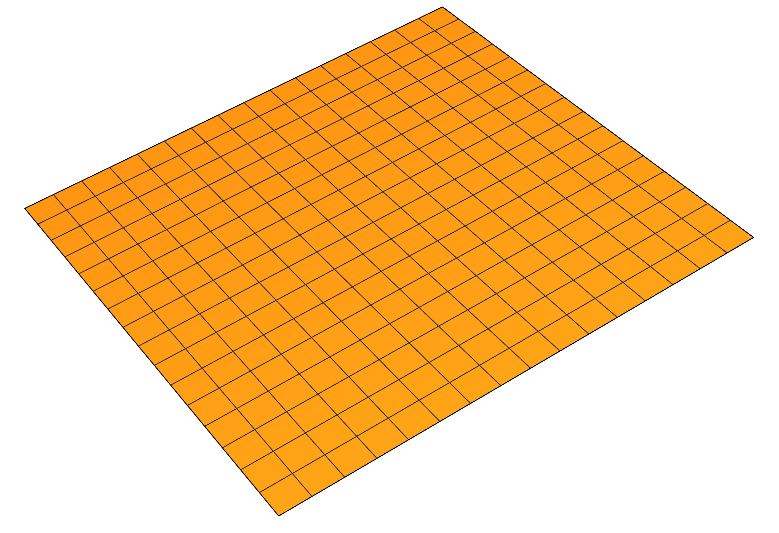
\includegraphics[width=\textwidth]{picture/week4/plane.pdf}
    \caption{Plane}
\end{subfigure}
\begin{subfigure}{0.2\textwidth}
    \centering
    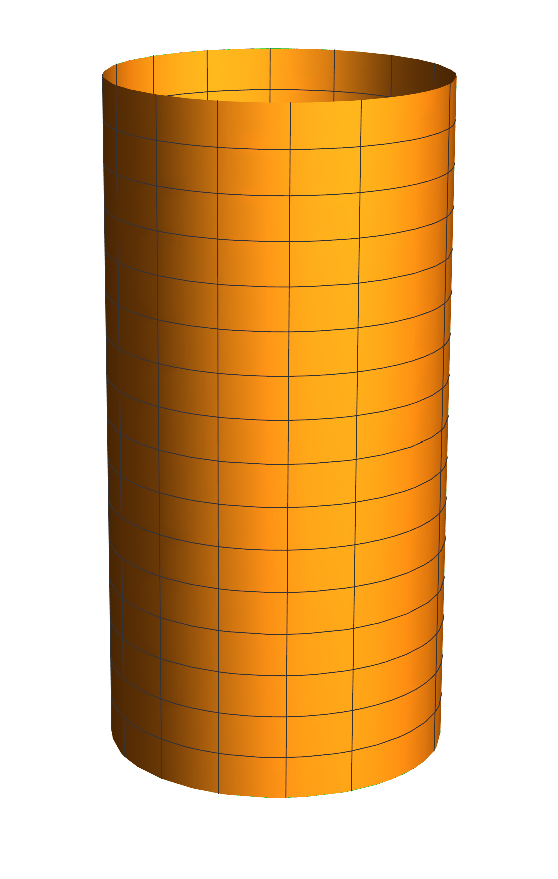
\includegraphics[width=\textwidth]{picture/week4/cylinder.pdf}
    \caption{Cylinder}
\end{subfigure}
\begin{subfigure}{0.4\textwidth}
    \centering
    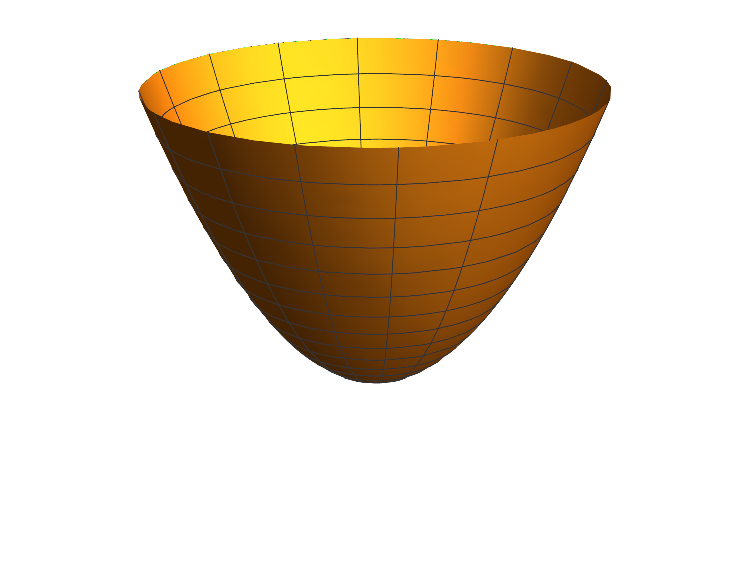
\includegraphics[width=\textwidth]{picture/week4/paraboloid.pdf}
    \caption{Paraboloid}
\end{subfigure}
\begin{subfigure}{0.3\textwidth}
    \centering
    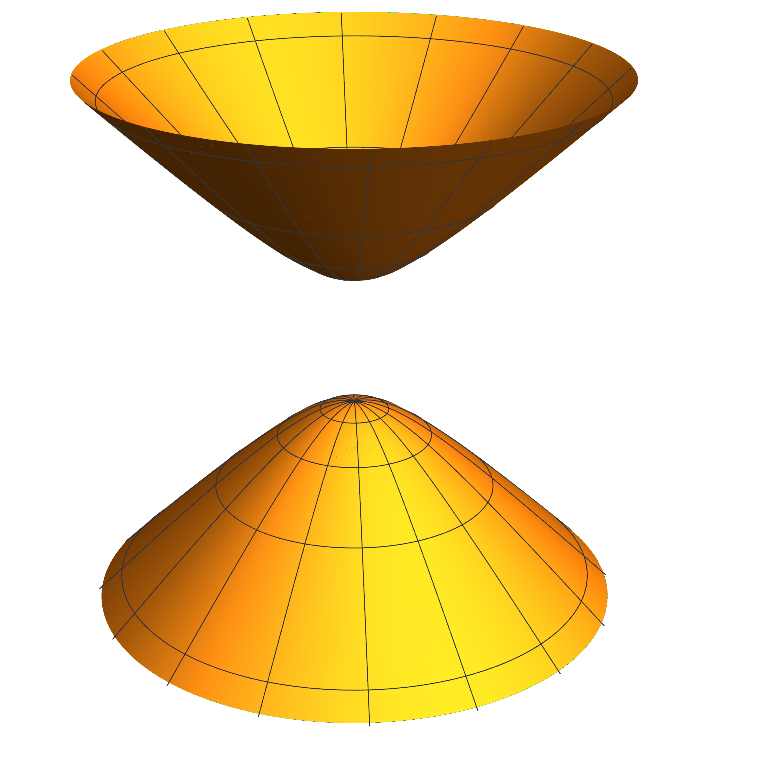
\includegraphics[width=\textwidth]{picture/week4/hyperboloid.pdf}
    \caption{Hyperboloid}
\end{subfigure}
\begin{subfigure}{0.2\textwidth}
    \centering
    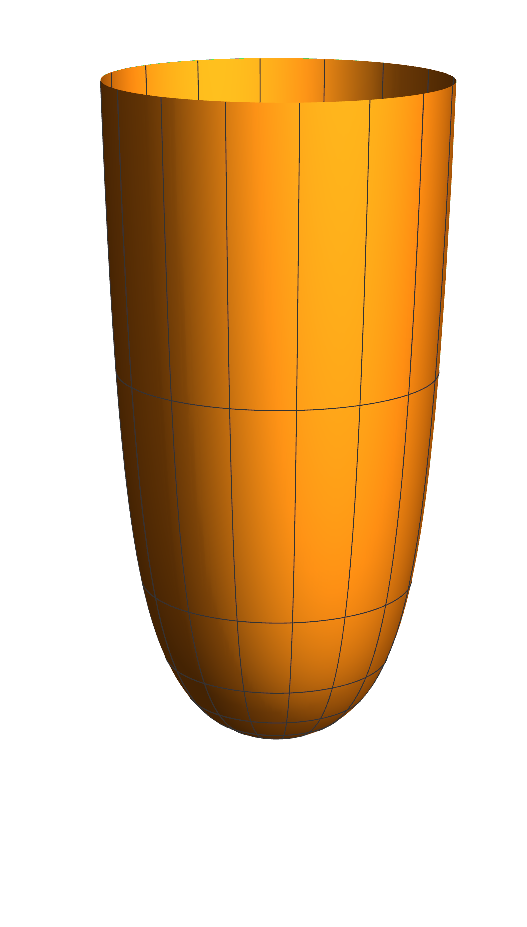
\includegraphics[width=\textwidth]{picture/week4/cigar.pdf}
    \caption{Cigar soliton}
\end{subfigure}
\caption*{Surface collection 1}
\end{figure}

\begin{figure}
\centering
\begin{subfigure}{0.25\textwidth}
    \centering
    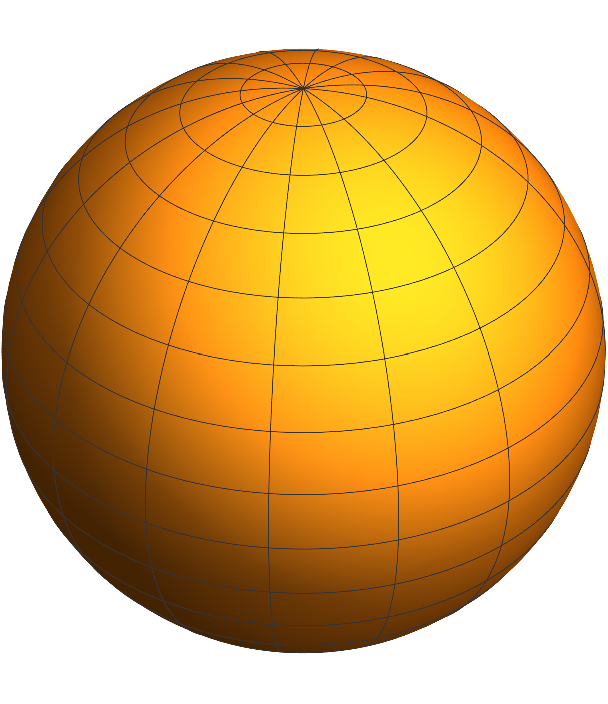
\includegraphics[width=\textwidth]{picture/week4/sphere.pdf}
    \caption{\(\mathbb{S}^2\)}
\end{subfigure}
\begin{subfigure}{0.35\textwidth}
    \centering
    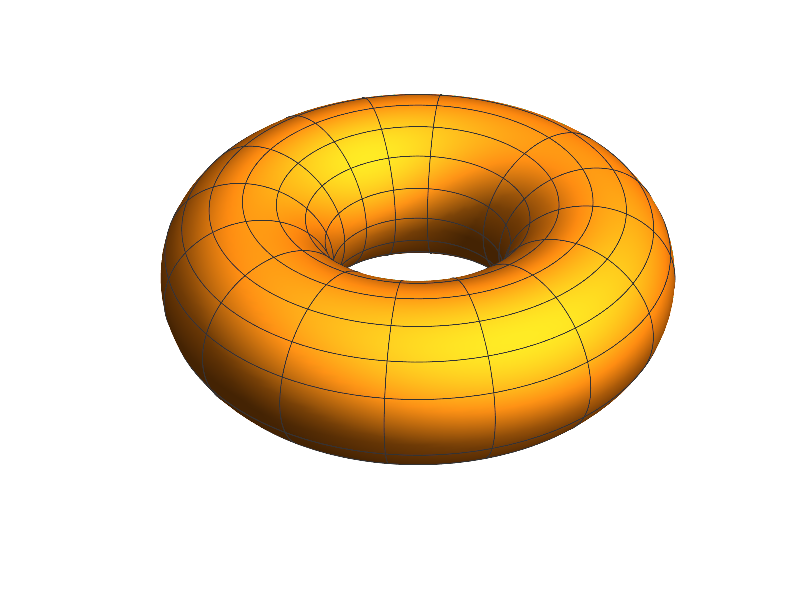
\includegraphics[width=\textwidth]{picture/week4/torus.pdf}
    \caption{\(\mathbb{T}^2\)}
\end{subfigure}
\begin{subfigure}{0.35\textwidth}
    \centering
    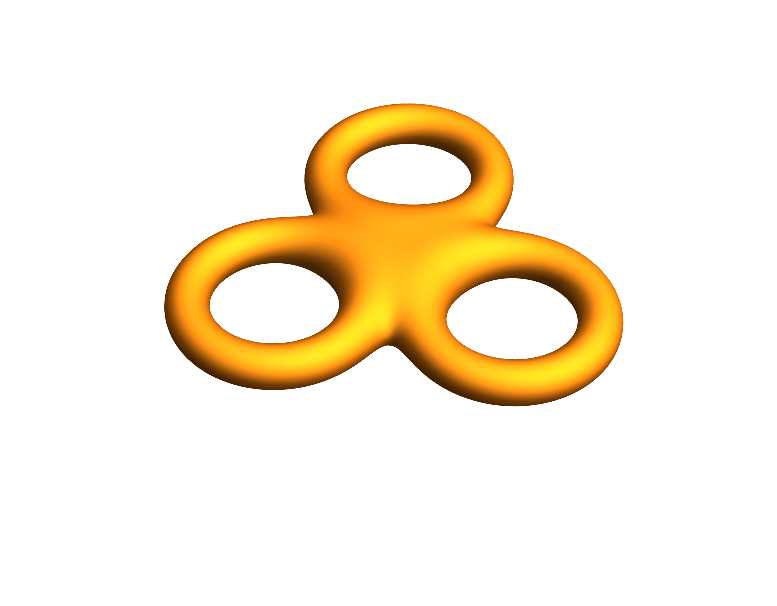
\includegraphics[width=\textwidth]{picture/week4/torus3.pdf}
    \caption{\(\Sigma_g\) for \(g=3\)}
\end{subfigure}
\caption*{Surface collection 2}
\end{figure}

\begin{figure}
\centering
\begin{subfigure}{0.45\textwidth}
    \centering
    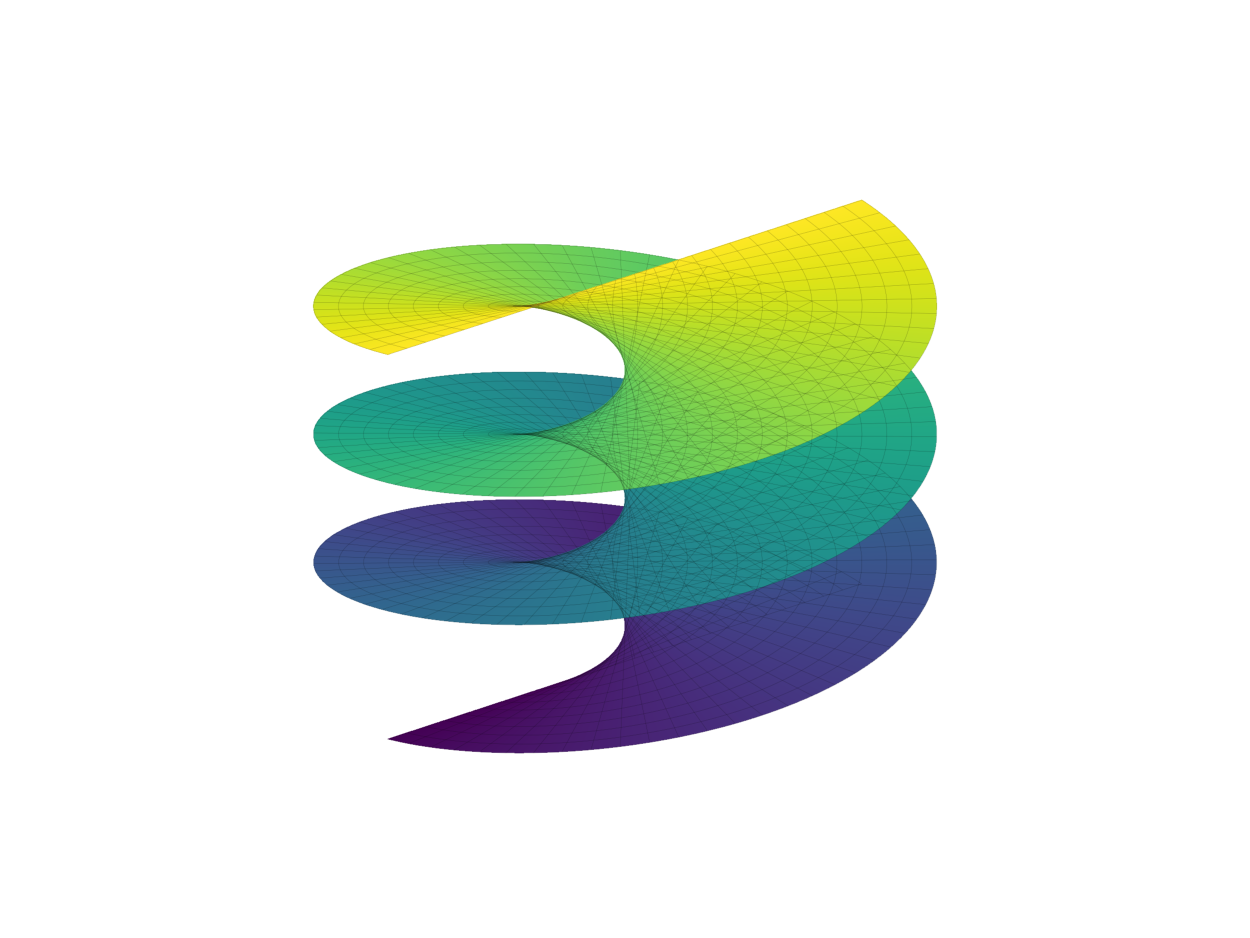
\includegraphics[width=\textwidth]{picture/week4/helicoid.pdf}
    \caption{Helicoid}
\end{subfigure}
\begin{subfigure}{0.45\textwidth}
    \centering
    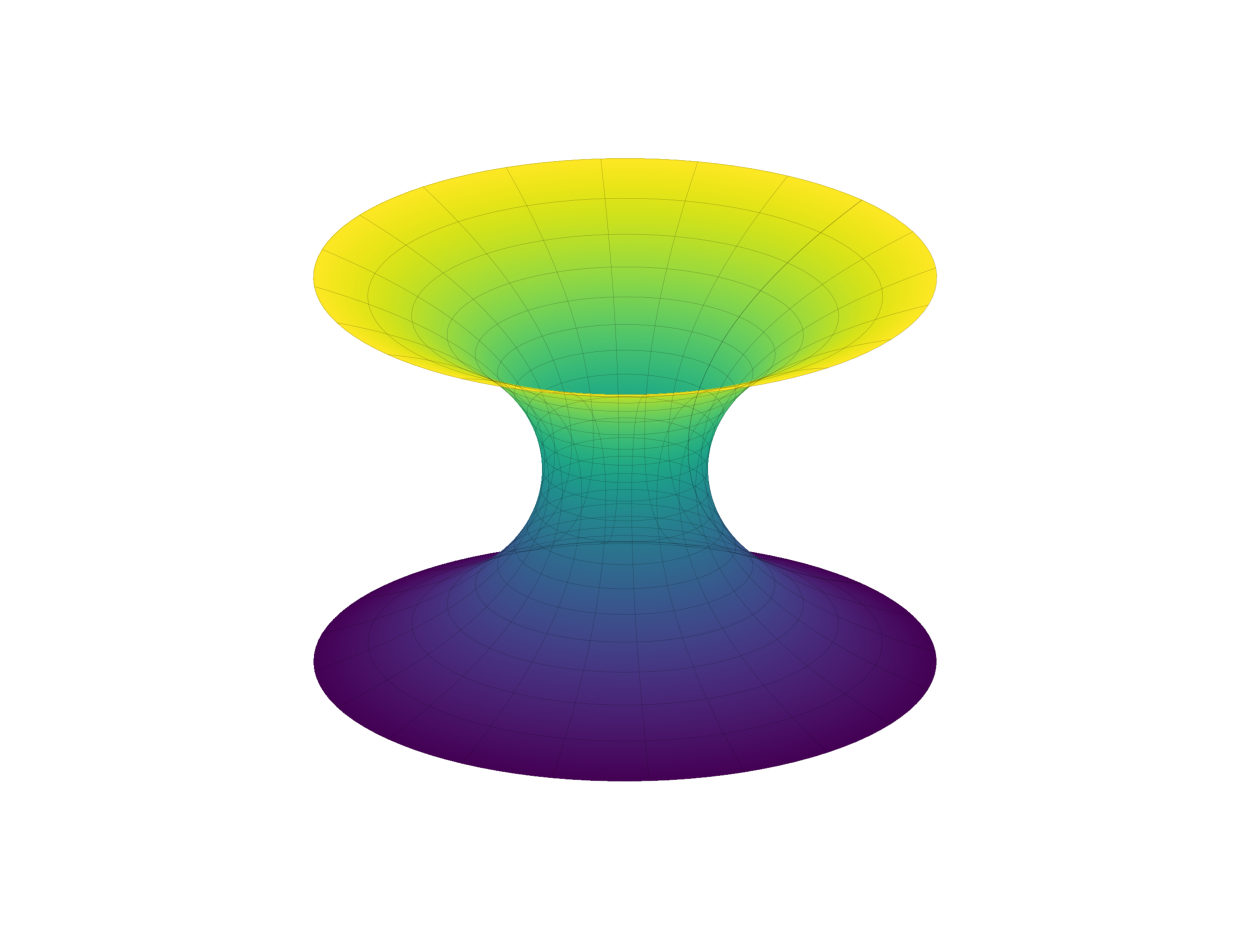
\includegraphics[width=\textwidth]{picture/week4/catenoid.pdf}
    \caption{Catenoid}
\end{subfigure}
\begin{subfigure}{0.5\textwidth}
    \centering
    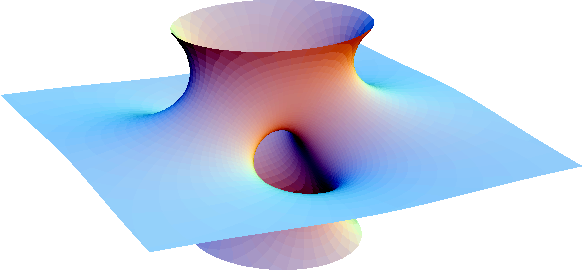
\includegraphics[width=\textwidth]{picture/week4/costa.pdf}
    \caption{Costa minimal surface}
\end{subfigure}
\begin{subfigure}{0.4\textwidth}
    \centering
    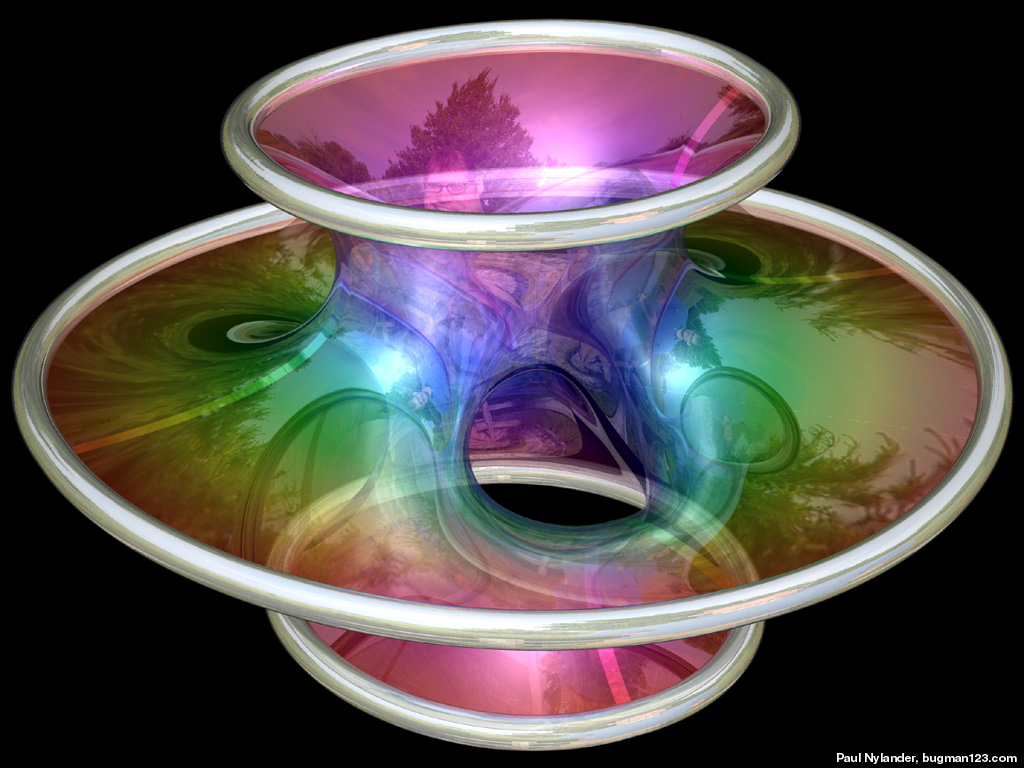
\includegraphics[width=\textwidth]{picture/week4/Costa-large.jpg}
    \caption{Soap bubble}
\end{subfigure}
\caption*{Surface collection 3}
\end{figure}

\begin{figure}
\centering
\begin{subfigure}{0.3\textwidth}
    \centering
    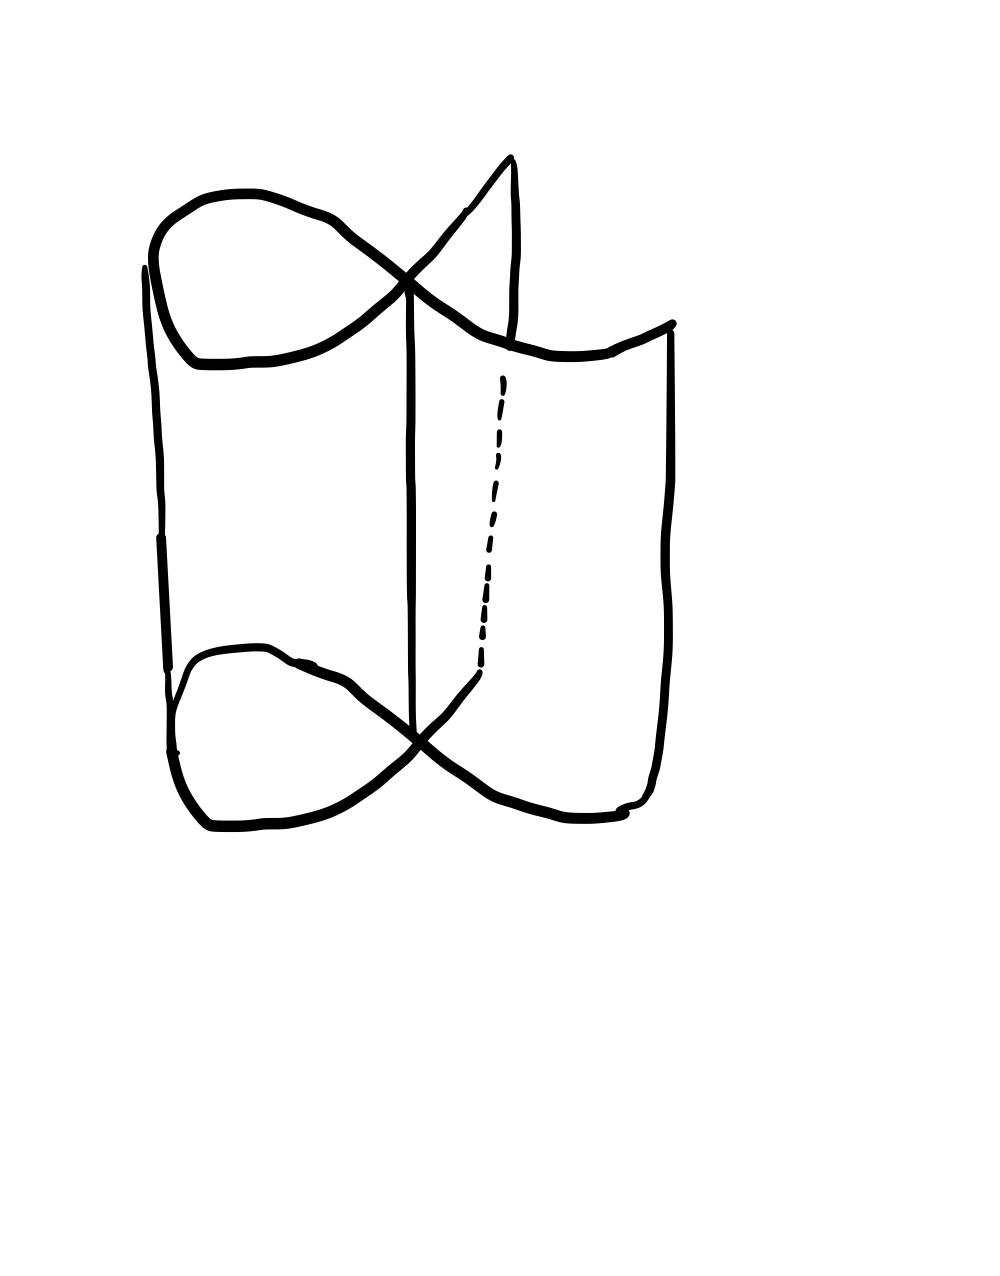
\includegraphics[width=\textwidth]{picture/week4/self-intersetcion.png}
    \caption{Self-intersected}
\end{subfigure}
\begin{subfigure}{0.35\textwidth}
    \centering
    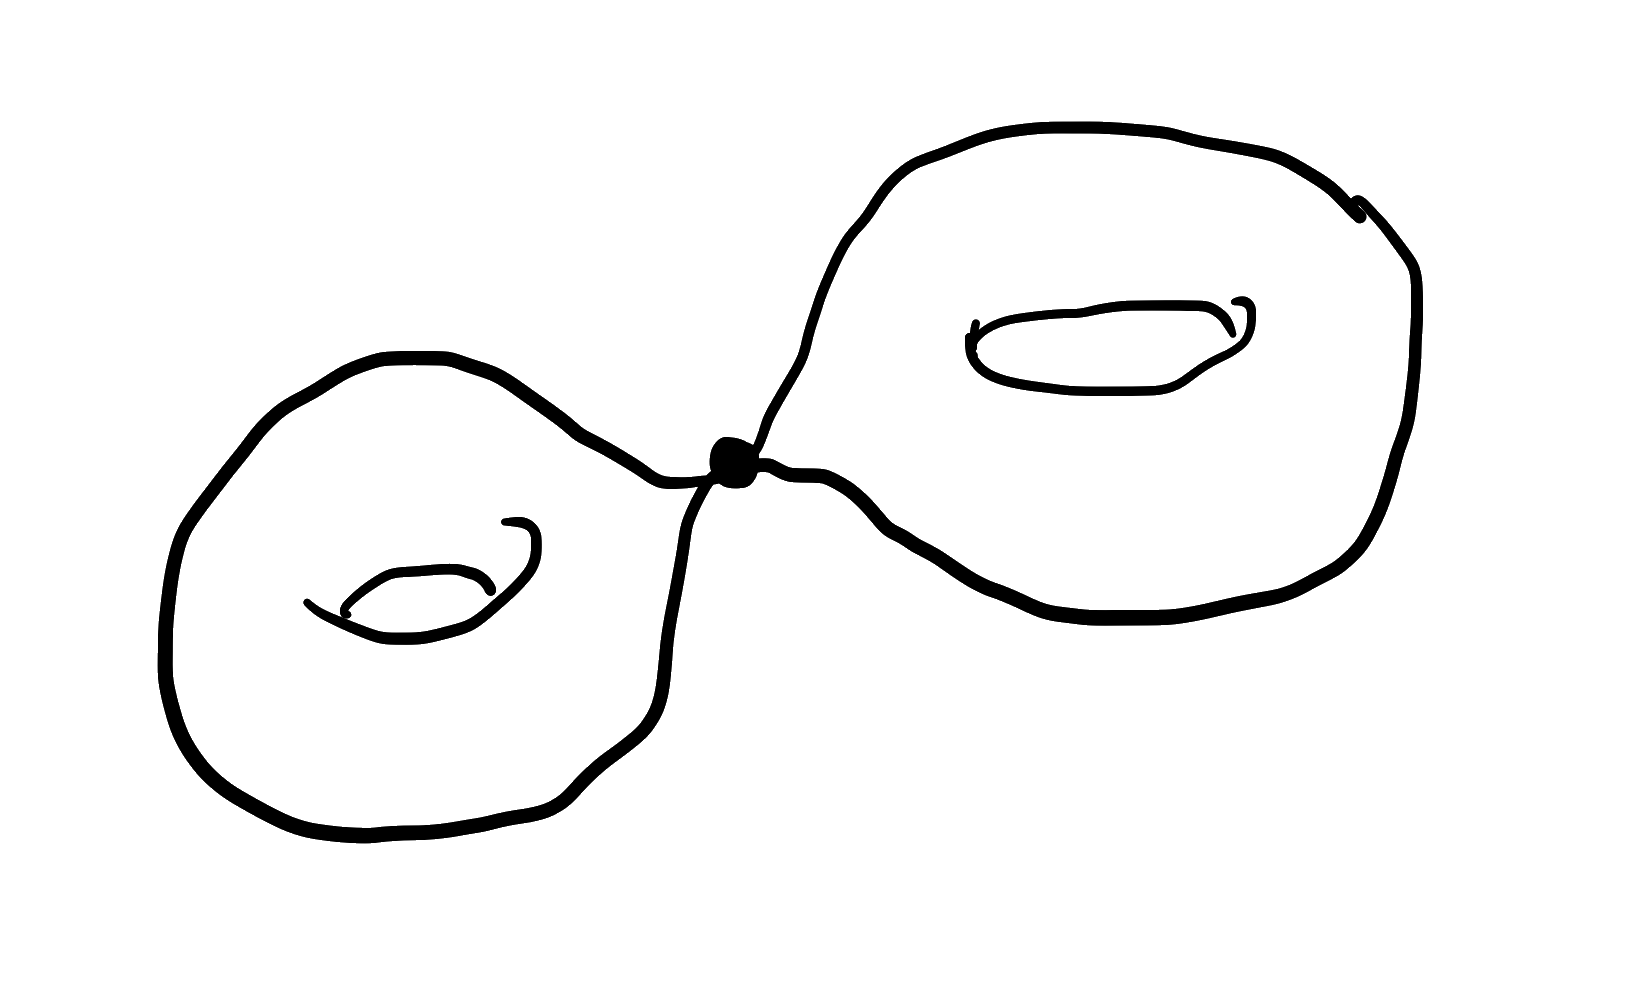
\includegraphics[width=\textwidth]{picture/week4/node.png}
    \caption{Nodal surfaces}
\end{subfigure}
\begin{subfigure}{0.3\textwidth}
    \centering
    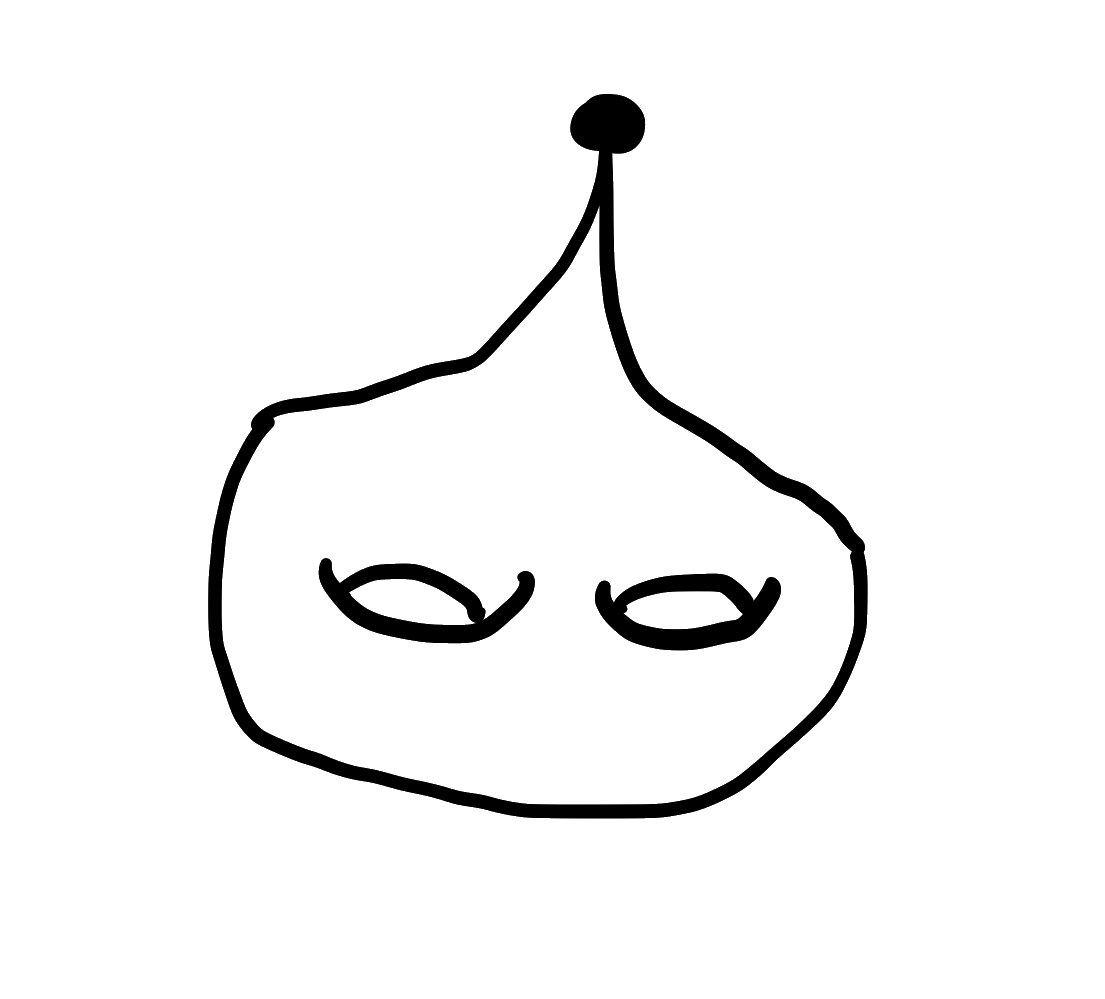
\includegraphics[width=\textwidth]{picture/week4/cusp.png}
    \caption{Cusp}
\end{subfigure}
\caption*{``Surface'' collection 4}
\end{figure}

\begin{example}\hfill
\begin{itemize}
    \item Collection 1 are complete non-compact surfaces.
    \item Collection 2 are compact surfaces without boundary (closed).
    \item Collection 3 are so called minimal surfaces, a very important class
        of surfaces. The term ``minimal'' intuits smallest area in certain sense.
    \item There are surfaces will NOT be investigated in this course, the ones with
        self-intersection, node points or cusps, and non-orientable surfaces.
\end{itemize}    
\end{example}

\section{Definition of Regular Surface}

\begin{definition}[Regular surfaces in \(\mathbb{R}^3\)]\hfill\par
    A subset \(S\subset \mathbb{R}^3\) is called a regular surface, if \(\forall\,p
    \in S\), \(\exists\, V\subset\mathbb{R}^3\) neighborhood of \(p\), an open set
    \(U\subset \mathbb{R}^2\) and a trivialization map \[
        F\colon U\to V\cap S
    .\] \st\ \(F\) is smooth, homeomorphism onto its image, and regular.
\end{definition}
\begin{remark}\hfill
\begin{enumerate}[(1)]
    \item \(F\) is homeomorphism means both \(F\) and \(F^{-1}\) are continuous map.
    \item \(F\) is ``regular'' means \(\forall\,p\in U\), \(\dif F_p\) is an 
        injection as linear map \(\mathbb{R}^2\to \mathbb{R}^3\).
\end{enumerate}
\end{remark}

Let's see what the term ``regular'' means:

Assume \(F\) is written as \(F(u,v)=(x(u,v),y(u,v),z(u,v))\), at \(p\in U\), \[
    \dd{F_p}\colon T_p U\to T_{F(p)}S
\] is a linear map. On \(\mathbb{R}^2\), coordinate vector fields \(\{\pdv{u},
\pdv{v}\}\) form a basis. On \(\mathbb{R}^3\) we also have standard basis
\(\{\pdv{x},\pdv{y},\pdv{z}\}\). Then \[
    \dd{F_p}\begin{bmatrix}
        \pdv{u}\\ \pdv{v}
    \end{bmatrix}
    =\begin{bmatrix}
        \pdv{x}{u} & \pdv{y}{u} & \pdv{z}{u} \\ 
        \pdv{x}{v} & \pdv{y}{v} & \pdv{z}{v}
    \end{bmatrix}
    \begin{bmatrix}
        \pdv{x}\\ \pdv{y}\\ \pdv{z}
    \end{bmatrix}
.\] Hence
\begin{align*}
    \dd{F_p}\text{ is injective}
    \iff & \ker\dd{F_p}=0 \\
    \iff & \pdv{(x,y,z)}{(u,v)}\text{ has rank 2} \\
    \iff & \pdv{F}{u}\text{ \& }\pdv{F}{v}\text{ are linearly independent} \\
    \iff & \pdv{F}{u}\times \pdv{F}{v}\neq 0. \\
    & \text{\small\itshape\/ (Geometrically this defines the normal vector field} \\
    & \text{\small\itshape\/ of the tangent plane)} \\
    \iff & \text{ One of the following minors is non-zero:}\\
    & \quad\left|\pdv{(x,y)}{(u,v)}\right|,\quad\left|\pdv{(x,z)}{(u,v)}\right|,
    \quad\left|\pdv{(y,z)}{(u,v)}\right|
\end{align*}
{\small\itshape
    (Geometrically, this means \((u,v)\) can be viewed as coordinate at \(p\in S\)
    via \(F\). In fact, since ``\(\dd{F_p}\) is injective'' is an open condition,
    \((u,v)\) serves as a local coordinate chart in a neighborhood of \(p\))
}

We also call \(F\) to be a local parametrization of \(S\). Note that such \(F\)
is usually not globally defined.

From the definition, we see a regular surface in \(\mathbb{R}^3\) is characterized
by at each point, we can find a ``smooth'' slice chart in a neighbourhood of the
point. The term ``slice chart'' means coordinate chart with local part of the
surface containing in the chart as a slice.

\begin{question}
    Consider two points \(p,q\) on the surface, live close to each other. It might
    happen that their corresponding coordinate chart overlap. Then in the
    intersection of two charts, there are two different parametrizations. What
    relation between these two parametrizations should be?
\end{question}
% Figure here

Set-up: \(F_1\colon U_1\to V_1\cap S,\ (u,v)\mapsto F_1(u,v)\),\hfill \(F_2\colon
U_2\to V_2\cap S,\ (\alpha,\beta)\mapsto F_2(\alpha,\beta)\)

Let \(W=V_1\cap V_2\cap S\), since \(F_i\) is homeomorphism, \(F_1^{-1}(W)\subset U,
\ F_2^{-1}(W)\subset U_2\).

\noindent\underline{\textbf{Claim:}} (Very important).\par
\(G=F_2^{-1}\circ F_1\colon F_1^{-1}(W)\to F_2^{-1}(W)\) is a diffeomorphism,\ie\ 
both \(G\) and \(G^{-1}\) are smooth functions.

The importance of this claim leads us to give an intrinsic definition of a regular
surface \(S\). \ie\ a regular surface is obtained by padding up open sets in
\(\mathbb{R}^2\), in a smooth way. Later in differential geometry course, we'll
define a smooth manifold by such intrinsic definition. The diffeomorphism \(G\)
above is called the transition map. Different property of \(G\) determines different
structure. If \(G\) is only a homeomorphism, then \(S\) is a topological surface.
If \(G\) is a bi-holomorphism, then \(S\) is a complex surface.

The proof of the claim needs the inverse function theorem.
\begin{theorem}[Inverse function thm]
    \(U\subset \mathbb{R}^n\) open. \(F\colon U\to \mathbb{R}^n\) is a \(C^1\) map,
    \(p\in U\). If \(\dd{F_p}\colon \mathbb{R}^n\to \mathbb{R}^n\) is an isomorphism,
    then there is a neighbourhood of \(p\) and a neighbourhood of \(F(p)\).
    \st\ \(F\colon V\to W\) is invertible. Moreover \(F^{-1}\) is also \(C^1\). If
    condition is substituted to \(F\) smooth, then \(F^{-1}\) has same smoothness.
\end{theorem}

\begin{remark}
    From linear algebra, a linear operator on finite dimensional vector space
    is injective iff it's surjective. Hence it's sufficient to check \(\det(\dd{F_p})
    \neq 0\), \ie\ \(\dd{F_p}\) is non-singular.
\end{remark}

\textbf{\color{red}!!} Apriori, we don't know if \(F_2^{-1}\) is smooth, since we
have not defined what ``smooth map'' on a surface mean.

\begin{proof}[Proof of claim]
    Since \(F_1\) and \(F_2\) are homeomorphism, \(G,G^{-1}\) are continuous.
    \(S\) is a regular surface, so at \(p\in U_1\), \((\dd{F_1})_p\colon\mathbb{R}^2
    \to \mathbb{R}^3\) is injective. W.L.O.G. we can assume \[
        \left|\pdv{(x,y)}{(u,v)}\right|\neq 0\text{ at }p
    .\] Consider a map \(h\colon F_1^{-1}(W)\times (-\eps,\eps)\to \mathbb{R}^3,
    (u,v,t)\mapsto (x(u,v),y(u,v),z(u,v)+t)\). Then \(h\) has Jacobian \[
        \det \begin{bmatrix}
            x_u & y_u & z_u \\
            x_v & y_v & z_v \\
            0 & 0 & 1
        \end{bmatrix}
        =\det\begin{bmatrix}
            x_u & y_u \\
            x_v & y_v 
        \end{bmatrix}\neq 0 \text{ at }p
    .\] By inverse function theorem, \(\exists\) a neighbourhood \(D\subset
    \mathbb{R}^3\) of \((p,t)\) \st\ \(h\) is invertible on \(D\), and \(h^{-1}\)
    smooth. Now since \(F_1^{-1}\circ F_2=\eval{h^{-1}\circ F_2}_{t=0}\), and RHS
    is smooth, we conclude that \(F_1^{-1}\circ F_2\) is smooth. Similarly \(G^{-1}\)
    is smooth.
\end{proof}

Now we give an intrinsic definition (No need to assume \(S\subset \mathbb{R}^3\)).
\begin{definition}
    Topological space \(S\) (second countable, Hausdorff) is called a regular surface
    if \(S\) has a covering \(\{V_\alpha,f_\alpha\}\) \st\ 
    \begin{enumerate}[(1)]
        \item \(f_\alpha\colon V_\alpha\to f_\alpha(V_\alpha)\overset{\text{open}}
            \subset \mathbb{R}^2\) is a homeomorphism.
        \item If \(V_\alpha\cap V_\beta\neq \emptyset\), then \[
            f_\beta\circ f_\alpha^{-1}\colon f_\alpha(v_\alpha\cap V_\beta)\to 
            f_\beta(V_\alpha\cap V_\beta)
        \] is a diffeomorphism, called the transition map.
    \end{enumerate}
\end{definition}
\begin{remark}
    In higher dimension, this definition yields ``smooth manifold''.
\end{remark}
